\documentclass[prc,amsmath,twocolumn,superscriptaddress]{revtex4}
%\bibliographystyle{prsty}
\usepackage{gensymb}
\usepackage{graphicx,color}
\usepackage{amssymb}
\usepackage{enumerate}
\usepackage{verbatim}
\usepackage{natbib}


\begin{document}

  \newcommand {\nc} {\newcommand}
  \nc {\Sec} [1] {Sec.~\ref{#1}}
  \nc {\IR} [1] {\textcolor{red}{#1}} 

\title{PHY905 Project 2 - Jacobi Algorithm}


\author{Alaina~Ross}

\date{\today}

%%%%%%%%%%%%%%%%%%%%%%%%%%%%%%%%%%%%%%%%%%%%%%%%%%%%%%%%%%%%%%%%%%%%%%%%%%%%%%%%%%%%%%%%%%%%%%%%%%%%%%%%%%%%%%%%%%%%%%%%%%%%%%%%%%%

\begin{abstract}
 \noindent {\bf Background:}% To solve a differential equation computationally the derivative is approximated and a system of linear equations is solved instead. Such systems can be solved via matrix equations and Gauss elimination. \\
\\ {\bf Purpose:} %The goal of this work is to implement various Gauss elimination algorithms and study the accuracy and performance of each when applied to a system of equations which result from the Poisson equation with a given example from electromagnetism. \\
\\ {\bf Method:} %We use a general Gauss elimination algorithm as well as two for tridiagonal matrixes and one which uses LU decomposition. We inspect the time to solution for varying matrix sizes and compare to the analytic solution to evaluate the accuracy of the algorithms. \\ 
\\ {\bf Results:} %We find the most accurate matrix size is $10^5$ and the fastest algorithm for this matrix size is the tridiagonal algorithm. \\
 \\ {\bf Conclusions:} %Our results demonstrate the importance of choosing the right algorithm for the given physical situation.
\end{abstract}


\maketitle

%%%%%%%%%%%%%%%%%%%%%%%%%%%%%%%%%%%%%%%%%%%%%%%%%%%%%%%%%%%%%%%%%%%%%%%%%%%%%%%%%%%%%%%%%%%%%%%%%
\section{introduction}
\label{intro}
For a single electron in a harmonic oscillator potential, the radial Schr{\"o}dinger equation is given by:
\begin{gather}
\frac{\hbar}{2m}\left(\frac{1}{r^2}\frac{d}{dr}r^2\frac{d}{dr}-\frac{\ell(\ell+1)}{r^2}\right)R_n(r) \notag \\
+\frac{1}{2}m\omega^2r^2 R_n(r)=E_{n\ell}R_n(r)
\end{gather}
where $R_n(r)$ are the radial wave functions, $\omega$ is the oscillator frequency, and $E_{n\ell}$ is the energy for the given quantum numbers:
\begin{equation}
E_{n\ell}=\hbar\omega\left(2n+\ell+\frac{3}{2}\right) \quad n,\ell = 0,1,2...
\end{equation}

In this work we will focus on $\ell=0$. Then making the substitution $u_n(r)=rR_n(r)$ and $\rho=\alpha/r$ where $\alpha^4=\hbar^2/mk$ and $k=m\omega^2$ gives:
\begin{equation}
-\frac{d^2}{d\rho^2}u_n(\rho)+\rho^2u_n(\rho)=\frac{2m\alpha}{\hbar^2}E_{n}u_n(\rho).
\end{equation}
Simplifying further, we can introduce the variable $\lambda$ such that:
\begin{equation}
-\frac{d^2}{d\rho^2}u_n(\rho)+\rho^2u_n(\rho)=\lambda u_n(\rho).
\end{equation}
This equation can be solved analytically to give the eigenvalues $\lambda_0=3$, $\lambda_0=7$, and $\lambda_2=11$.

If rather than one electron in the harmonic oscillator well there are two which are non-interacting, then Equation 1 becomes:
\begin{gather}
\left(-\frac{\hbar^2}{2m}\frac{d^2}{dr_1^2}-\frac{\hbar^2}{2m}\frac{d^2}{dr_2^2}+\frac{1}{2}kr_1^2 +\frac{1}{2}kr_2^2 \right)u_n(r_1,r_2) \notag \\
= E_n^{(2)}u_n(r_1,r_2)
\end{gather}
where $u_n(r_1,r_2)$ is a two-body wave function and $E_n^{(2)}$ is the two-electron energy. We introduce new coordinates, \textbf{r} and \textbf{R}, defined by:
\begin{gather}
\mathbf{r}=\mathbf{r_1}-\mathbf{r_2} \\
\mathbf{R}=\frac{1}{2}\left(\mathbf{r_1}+\mathbf{r_2}\right) 
\end{gather}
where \textbf{r} is the relative coordinate and \textbf{R} is the relative center-of-mass coordinate. This simplifies Equation 5 to:
\begin{gather}
\left(-\frac{\hbar^2}{m}\frac{d^2}{dr^2}-\frac{h^2}{4m}\frac{d^2}{dR^2} + \frac{1}{4}kr^2+kR^2\right)u_n(r,R) \notag \\
=E_n^{(2)}u_n(r,R)
\end{gather}
and allows for the both the wave function and the energy to be written in terms of a relative wave function and energy, $\psi(r)$ and $E_r$, and a center-of-mass wave function and energy, $\phi(R)$ and $E_R$:
\begin{gather}
u(r,R)=\psi(r)\phi(R) \\
E^{(2)}=E_r+E_R.
\end{gather}

This change of variables proves even more useful though when a repulsive Coulomb interaction is included as:
\begin{equation}
V(r_2,r_2)=\frac{\beta e^2}{|\mathbf{r}_1-\mathbf{r}_2|}=\frac{\beta e^2}{r}
\end{equation}
where $\beta e^2$ = 1.44 eVnm. As this potential only depends on the relative coordinate, we can look exclusively at the Schr{\"o}dinger equation for the relative wave function:
\begin{equation}
\left(-\frac{h^2}{m}\frac{d^2}{dr^2}+\frac{1}{4}kr^2+\frac{\beta e^2}{r}\right)\psi(r)=E_r\psi(r).
\end{equation}

Again we can make the substitution $\rho=r/\alpha$ where now $\alpha=\hbar^2/m\beta e^2$. In addition, we introduce the frequency $\omega_r=mk\alpha^4/4\hbar^2$, which reflects the strength of the oscillator potential, and the variable $\lambda = m\alpha^2E_r/\hbar^2$. Equation 12 then becomes:
\begin{equation}
-\frac{d^2}{d\rho^2}\psi(\rho)+w_r^2\rho^2\psi(\rho)+\frac{1}{\rho}=\lambda\psi(\rho).
\end{equation}
This equation has been solved analytically for some values of $\omega_r$ in~\cite{interact}. Of specific interest in this work is the case $\omega_r=0.05$, where the ground state eigenvalue is given by $\lambda=0.35$.

In this work we implement the Jacobi algorithm to solve the eigenvalue problems described above and study the performance characteristics and numerical accuracy for different grid and step sizes. In addition, we investigate the influence of the frequency $w_r$ on the shape of the wave functions in the interacting case. In Section~\ref{methods}, the implementation of the algorithm is described. In Section~\ref{results} the performance and accuracy of the code are analyzed. Finally, in Section~\ref{conc} we give a summary and our conclusions.

\section{methods}
\label{methods}

\section{results}
\label{results}
\begin{figure}[h]
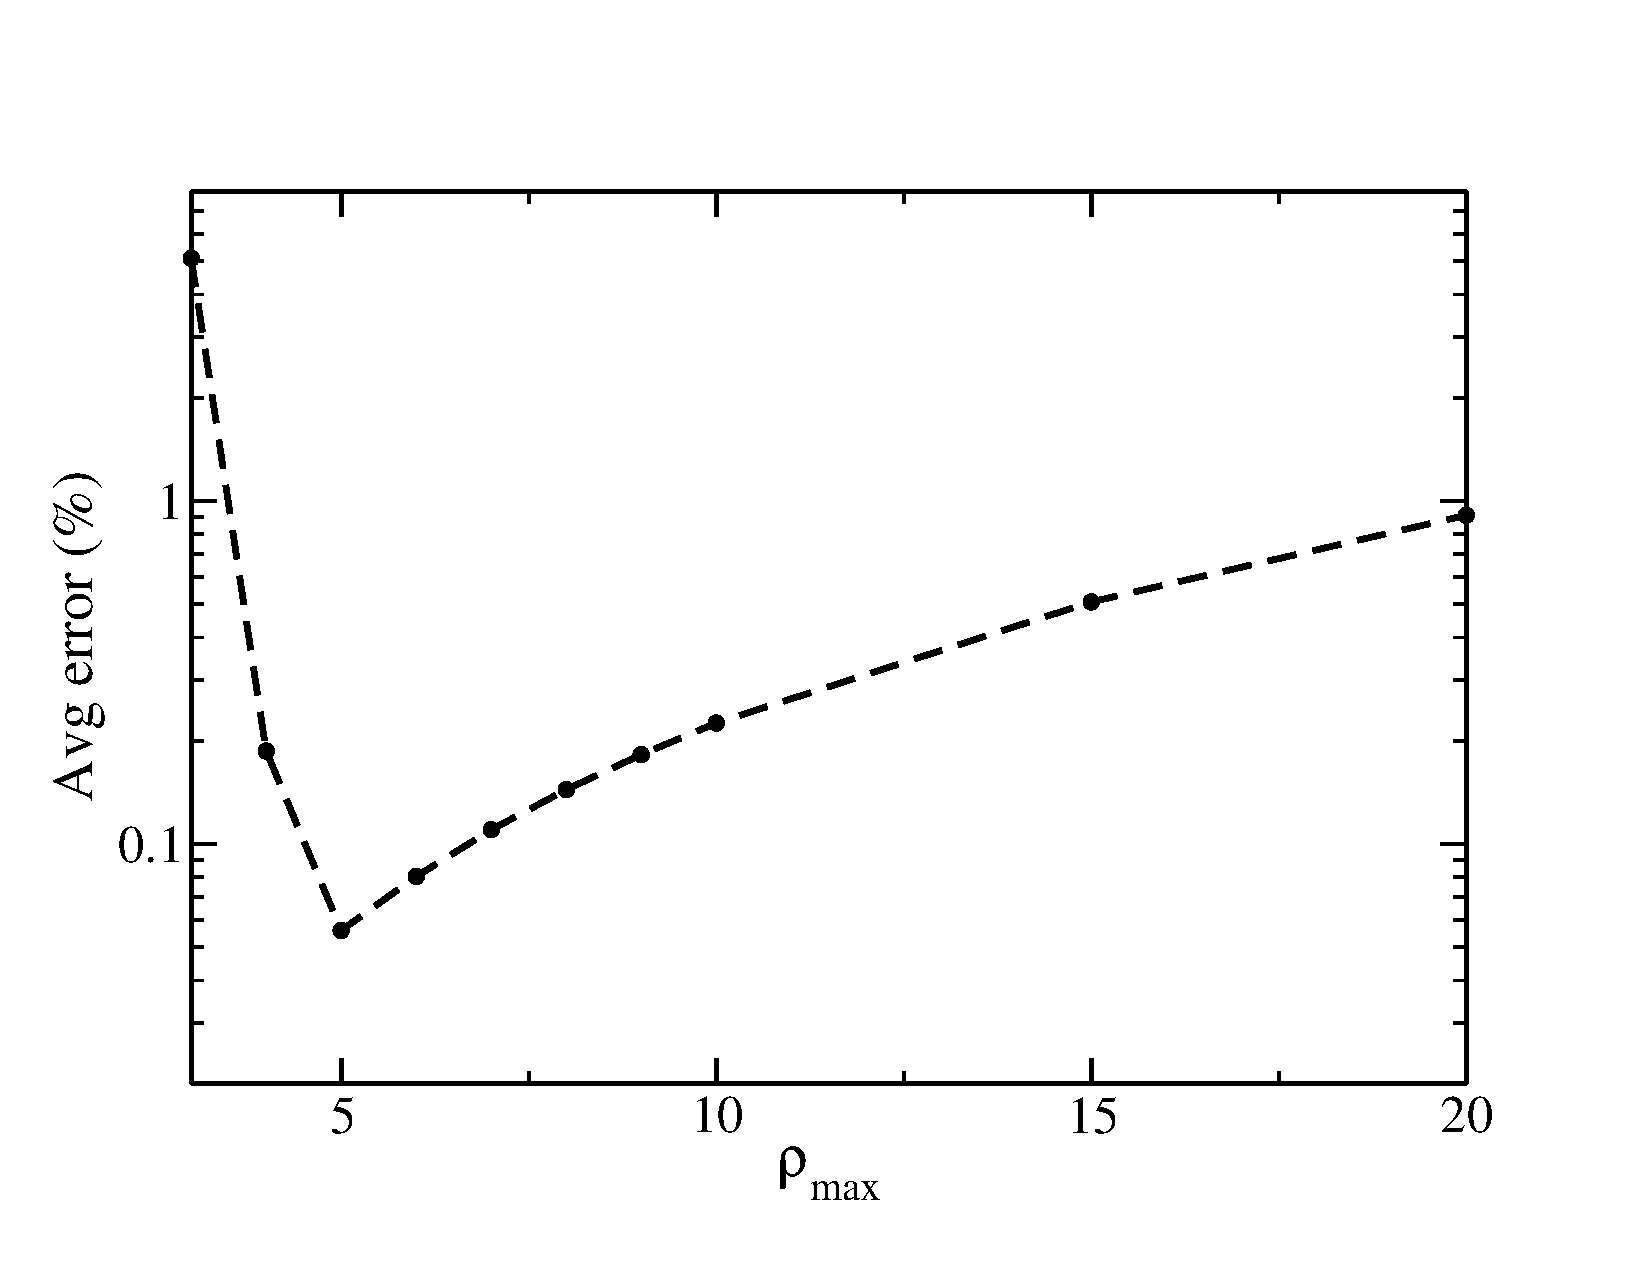
\includegraphics[scale=0.33]{error_pmax.pdf}
\caption{error asa function of $\rho_{max}$}
\label{algorithm}
\end{figure}

\begin{figure}[h]
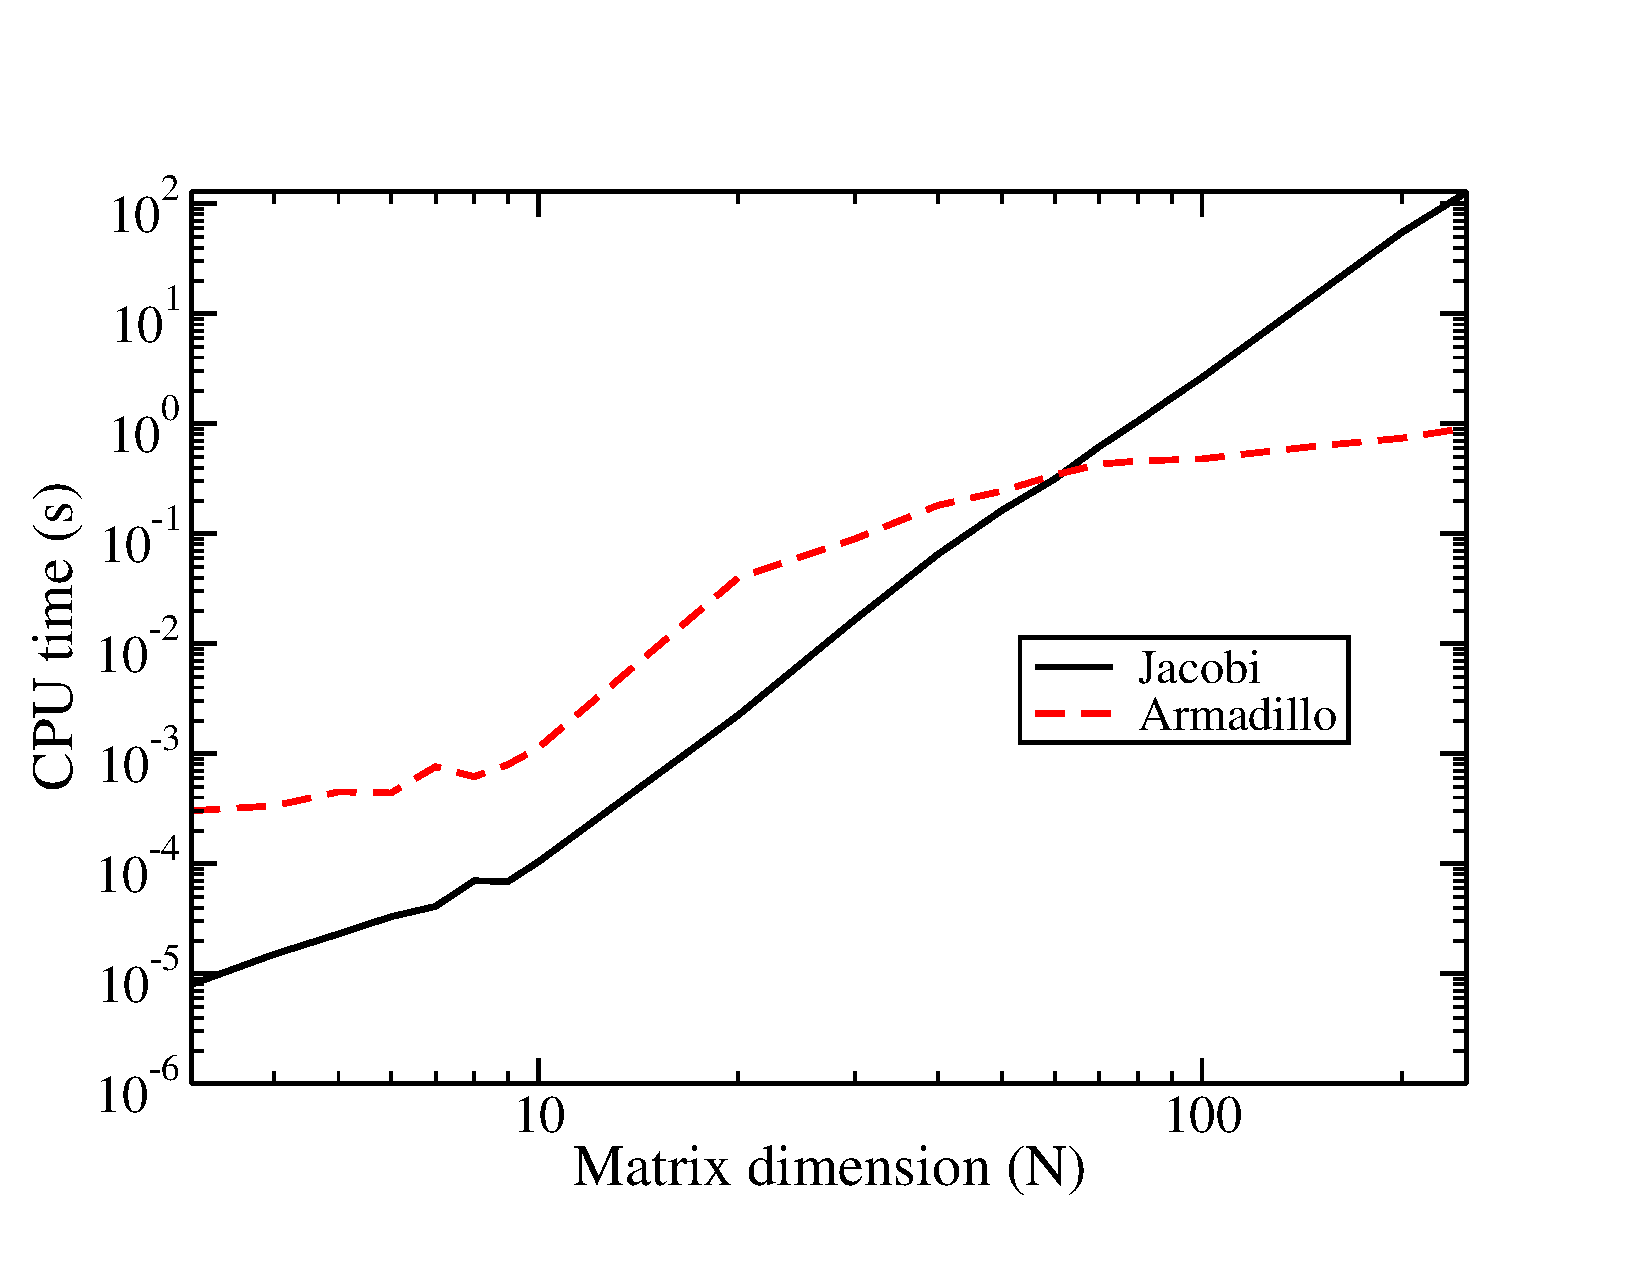
\includegraphics[scale=0.33]{N_time2.pdf}
\caption{time as a function of matrix dimension (N)}
\label{algorithm}
\end{figure}

\begin{figure}[h]
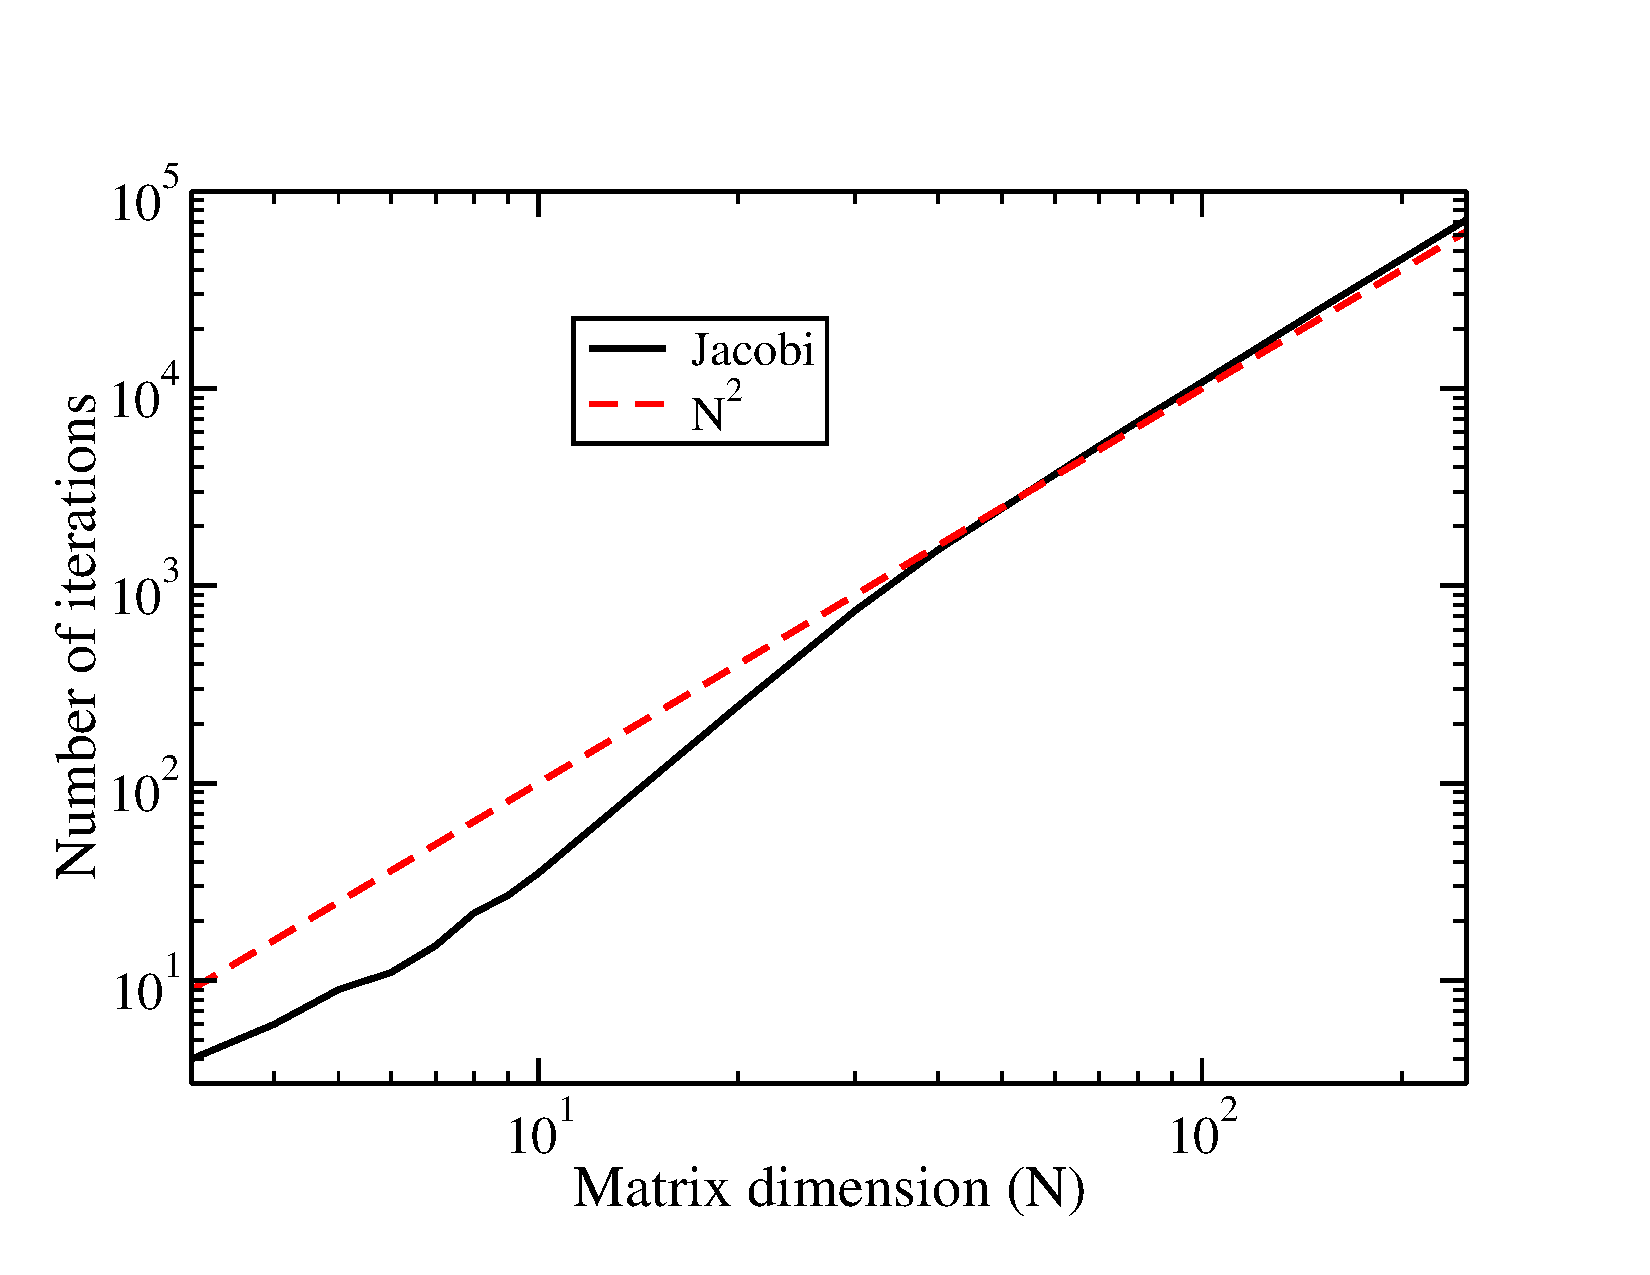
\includegraphics[scale=0.33]{N_trans.pdf}
\caption{number of rotations as a function of matrix dimension (N)}
\label{algorithm}
\end{figure}

\begin{figure}[h]
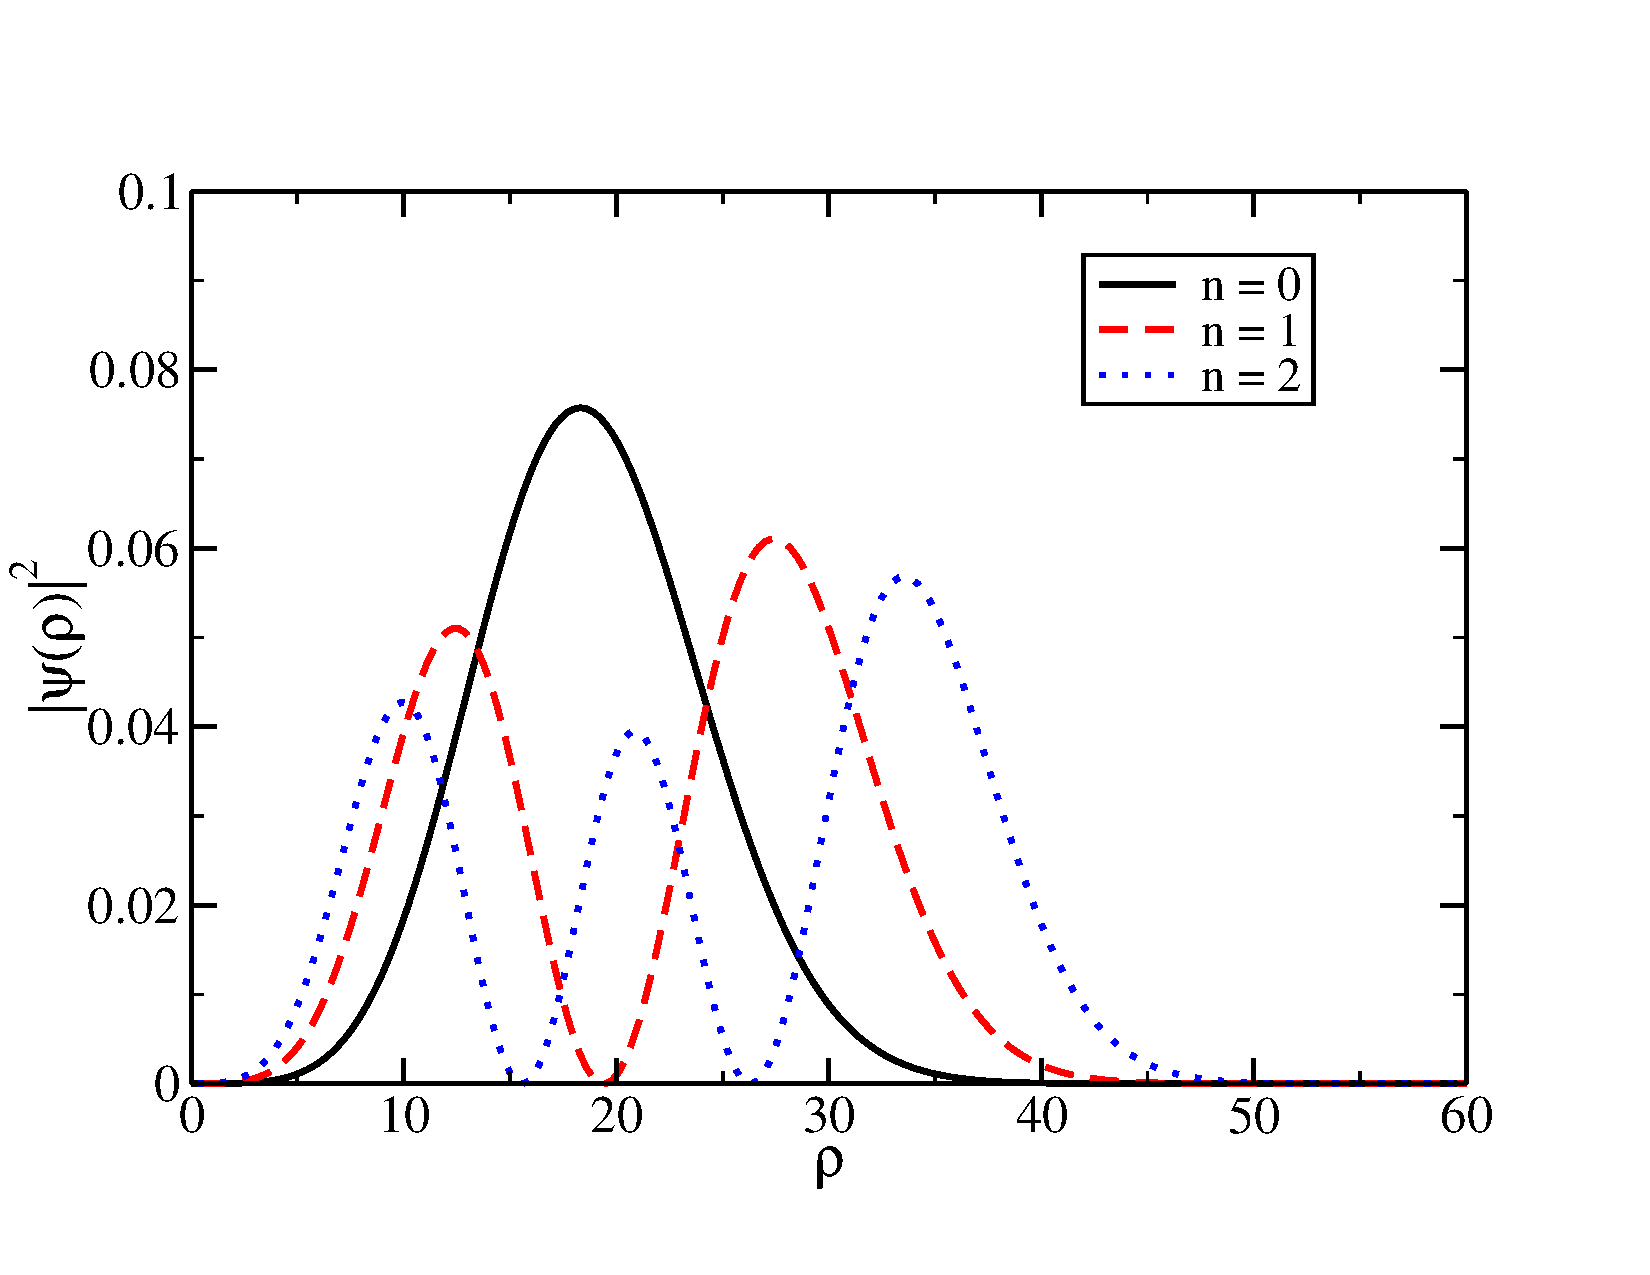
\includegraphics[scale=0.33]{wf_01.pdf}
\caption{$|u(\rho)|^2$ for $w_r = 0.01$}
\label{algorithm}
\end{figure}

\begin{figure}[h]
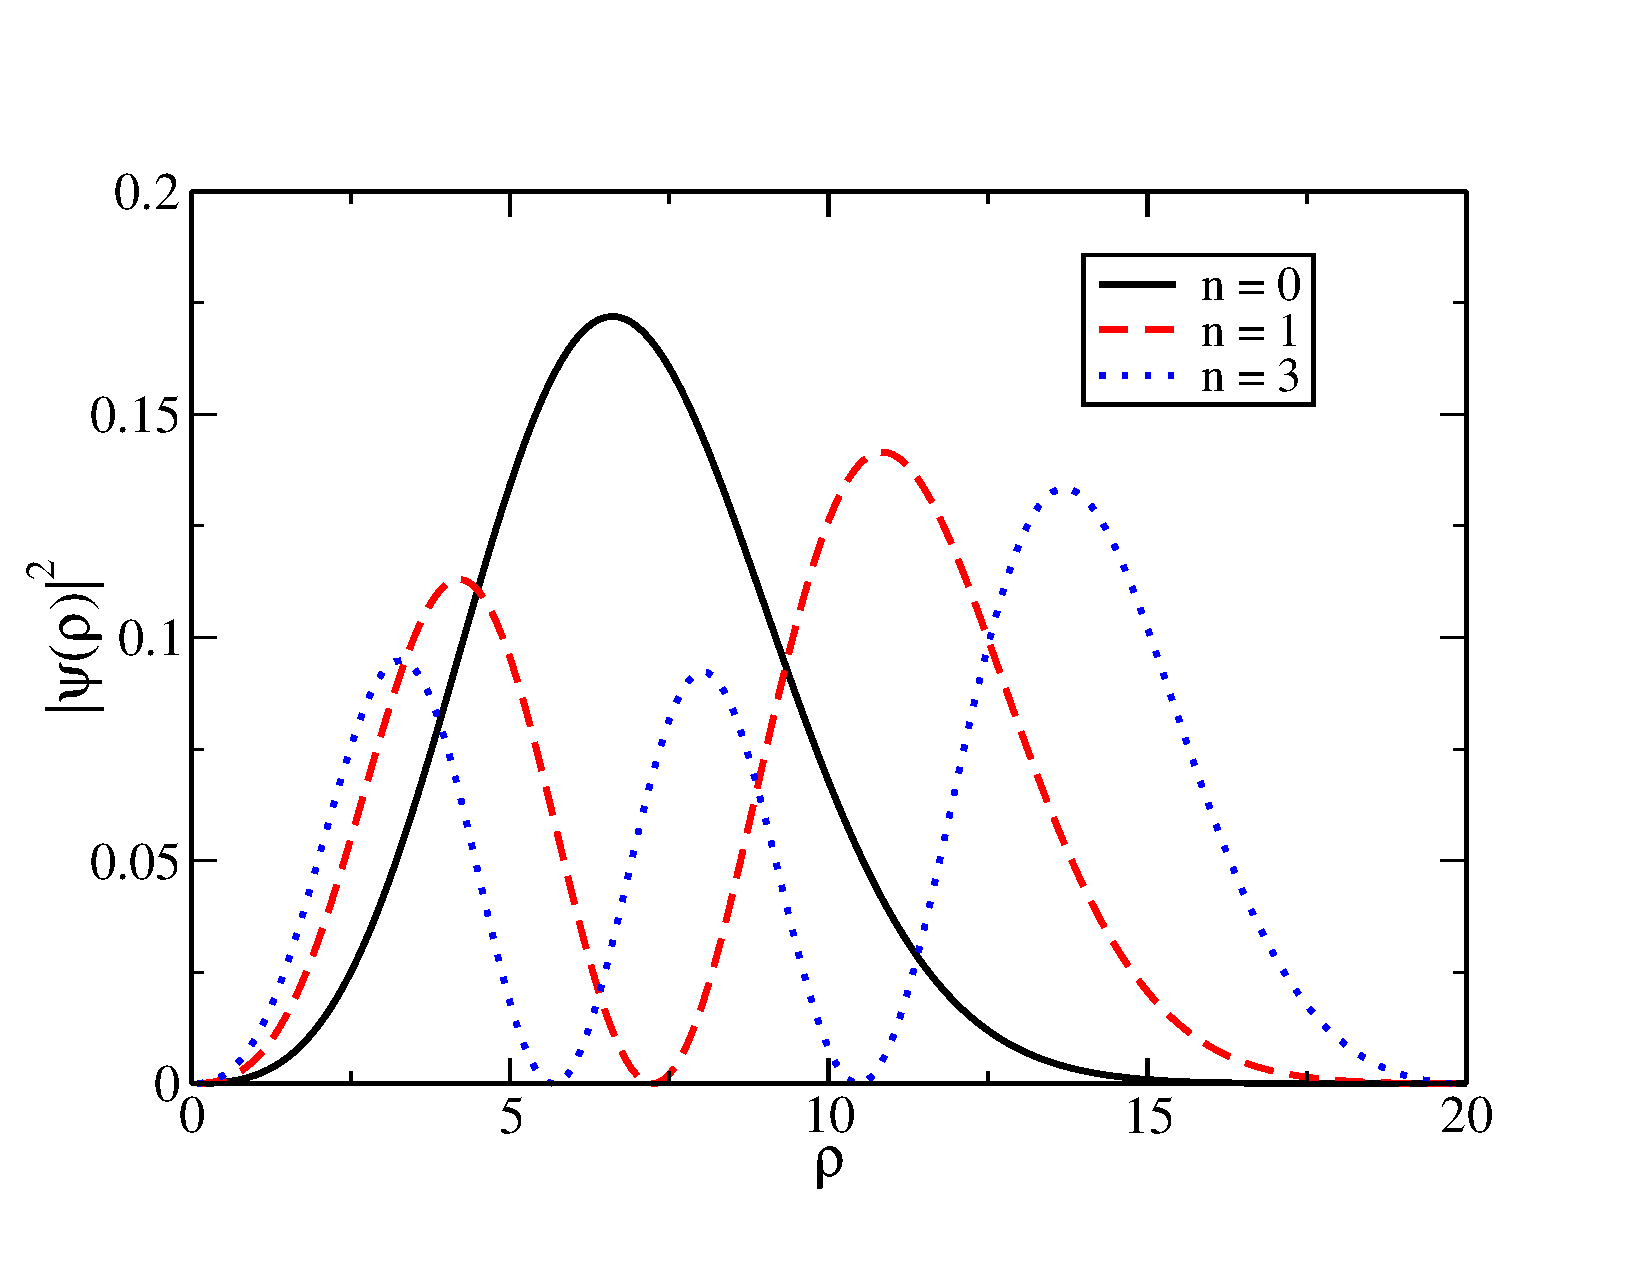
\includegraphics[scale=0.33]{wf_05.pdf}
\caption{$|u(\rho)|^2$ for $w_r = 0.05$}
\label{algorithm}
\end{figure}

\begin{figure}[h]
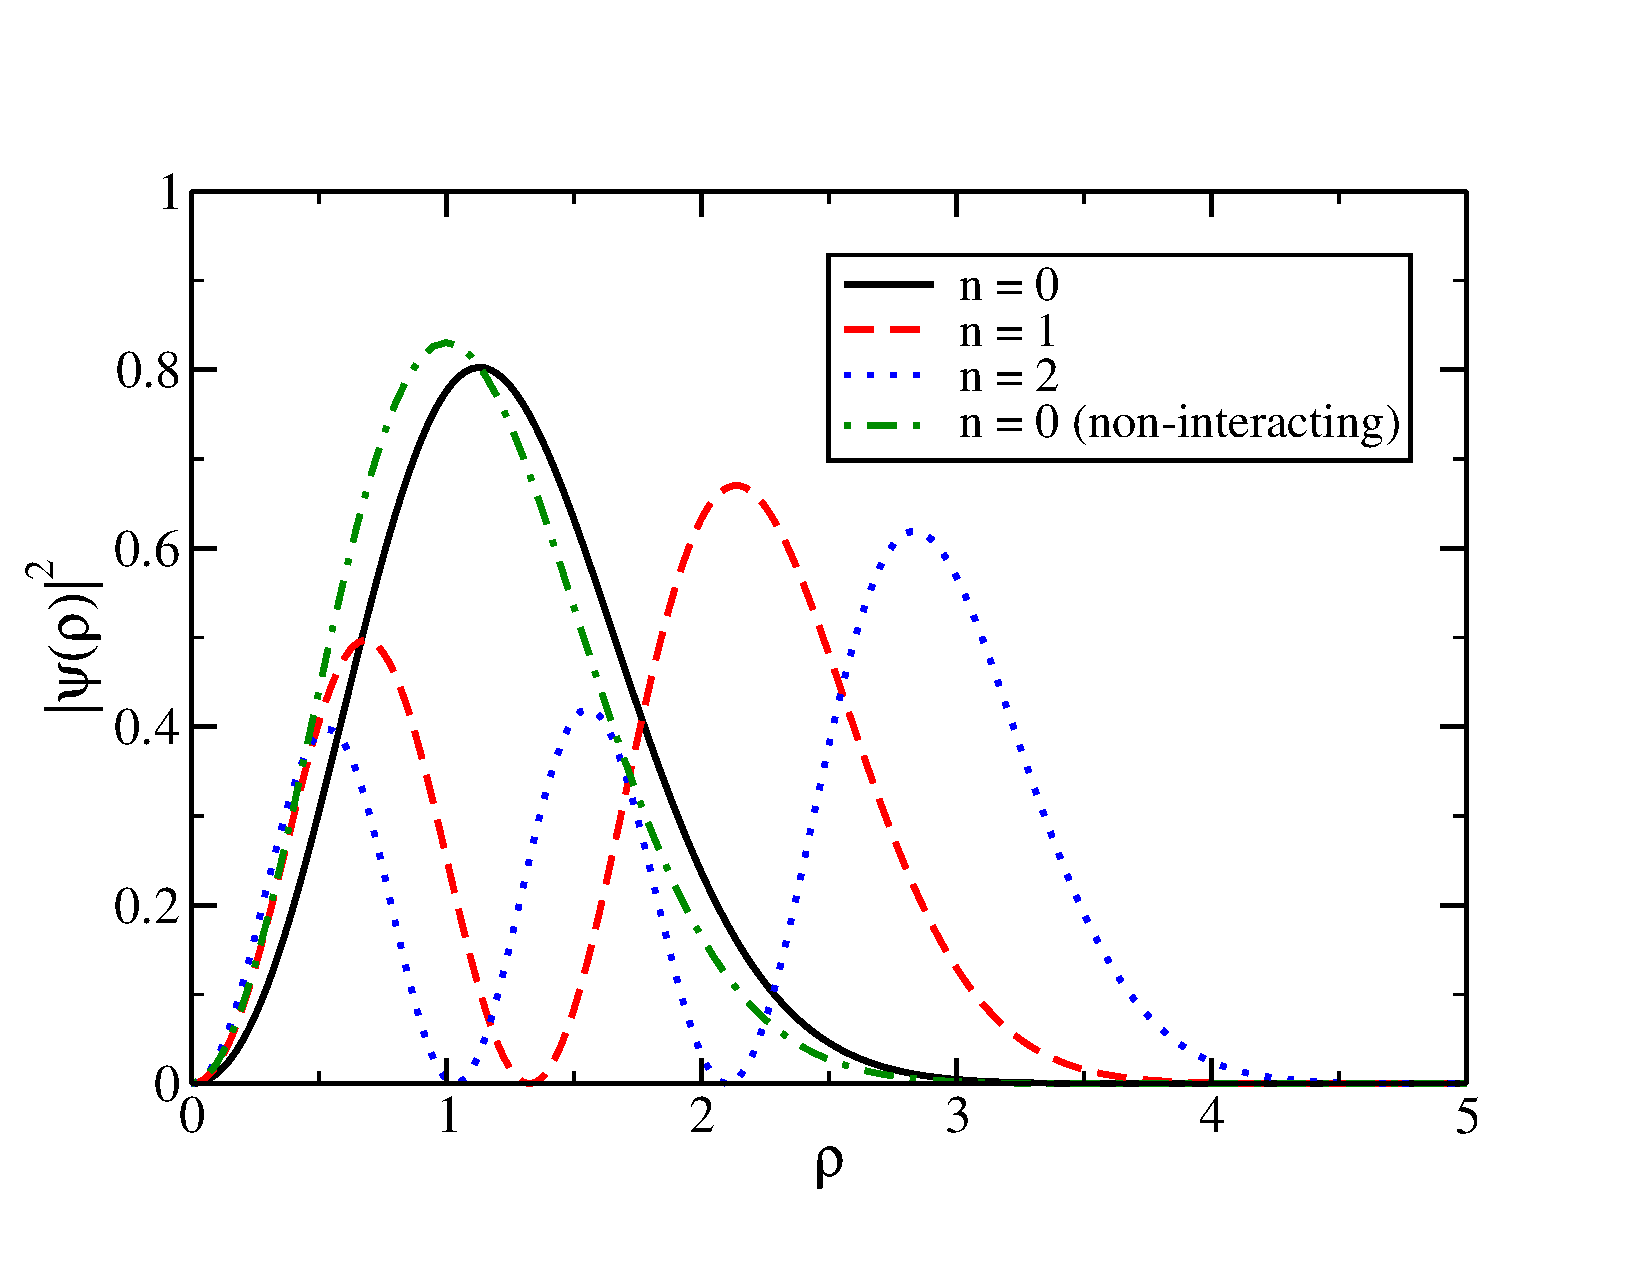
\includegraphics[scale=0.33]{wf_1.pdf}
\caption{$|u(\rho)|^2$ for $w_r = 1.0$}
\label{algorithm}
\end{figure}

\begin{figure}[h]
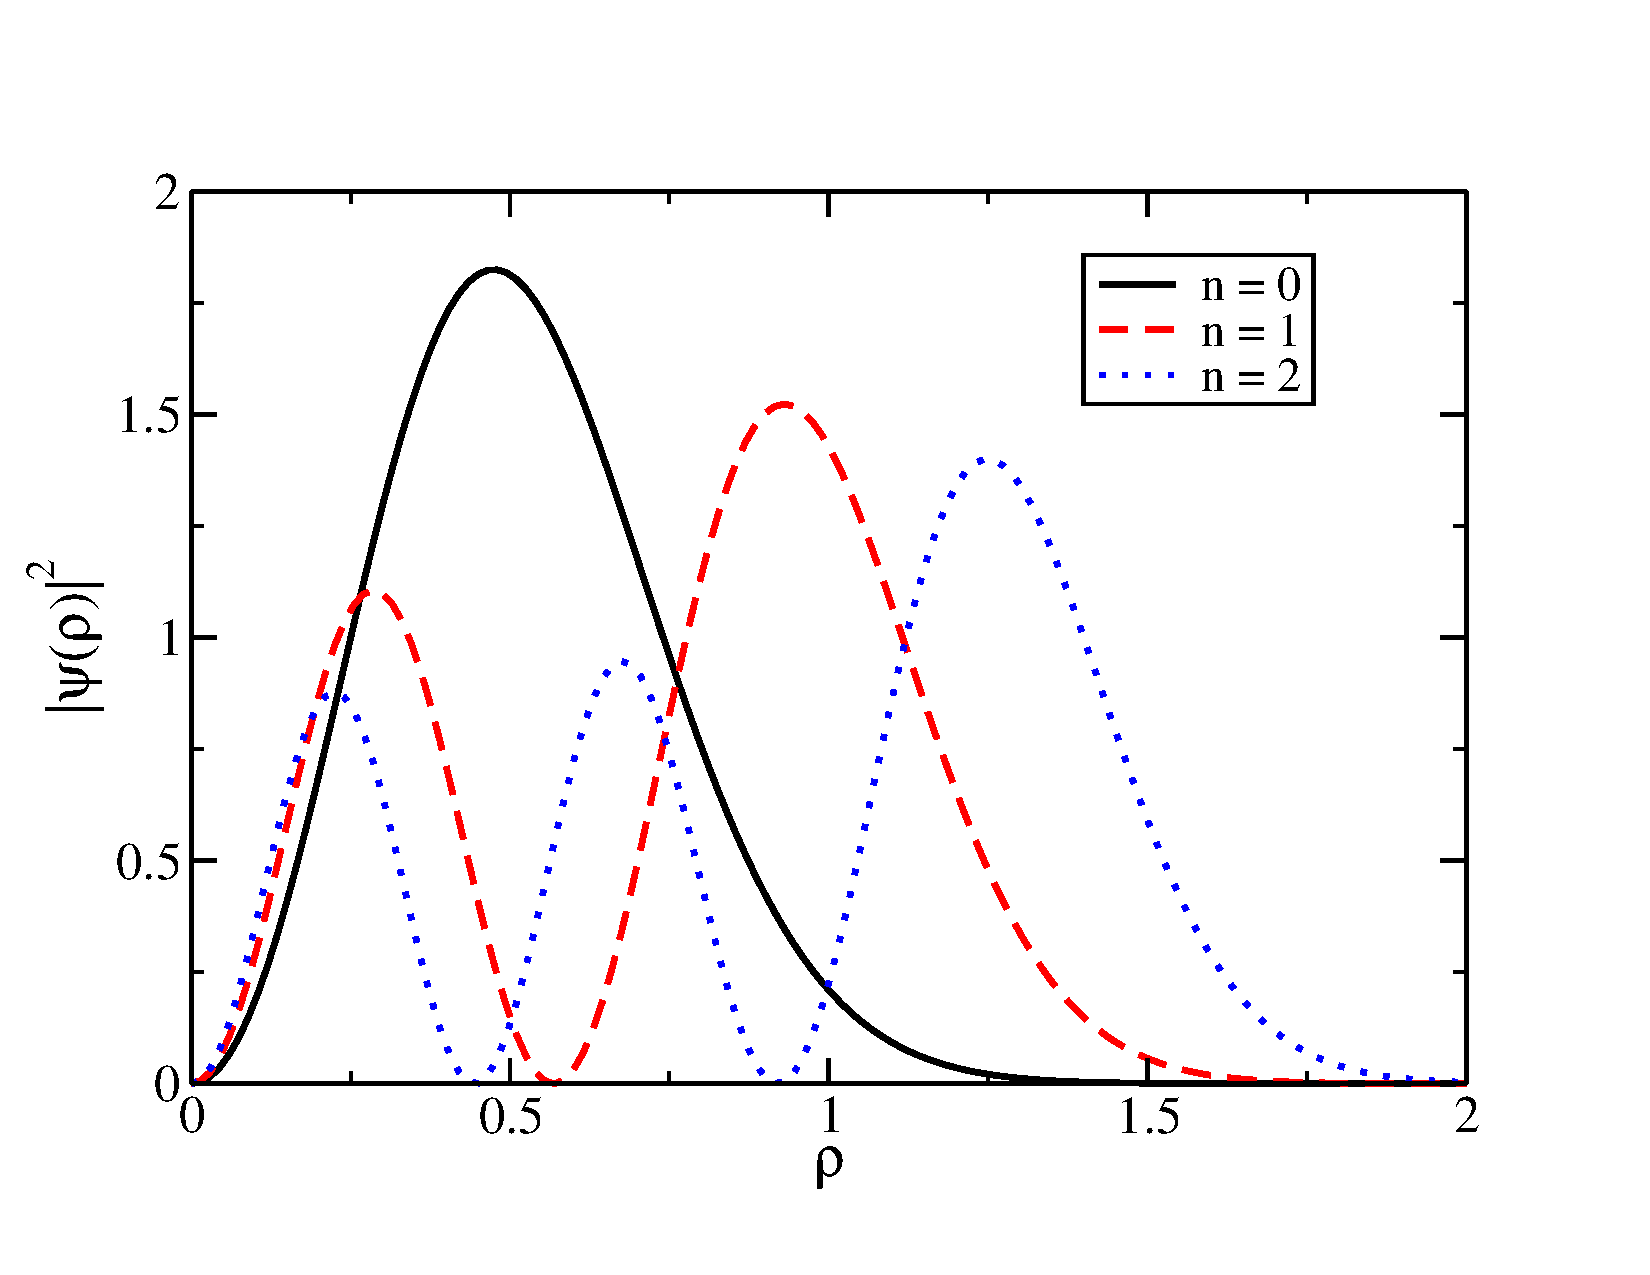
\includegraphics[scale=0.33]{wf_5.pdf}
\caption{$|u(\rho)|^2$ for $w_r = 5.0$}
\label{algorithm}
\end{figure}

%\begin{table}[b]
%\centering
%\begin{tabular}{|c|c|}
%\hline
%Algorithm& FLOPs\\
%\hline
%General Gauss&$\frac{2}{3}n^3$\\
%Tridiagonal matrix&$8n$\\
%Specific tridiagonal&$6n$\\
%LU  decomposition&$2n^2$\\
%\hline
%\end{tabular}
%\caption{Comparison of number of FLOPs for each algorithm.}
%\label{flop_table}
%\end{table}

\section{conclusions}
\label{conc}

\bibliography{jacobi}
\end{document}

